\section{A deterministic sum with a density in all coordinates}
\begin{proof}[Proof of Theorem~\ref{th:several}]
First, the sequence
\((\theta_{n^{\alpha_1}},\ldots,\theta_{n^{\alpha_m}})\) is equidistributed in \(H^m\).
A nontrivial product character has phase \(f(n)=\sum_j\omega_j n^{\alpha_j}\) with at least one nonzero \(\omega_j\). Let \(\alpha\) be the largest active exponent. On \([N,2N]\), for large \(N\), \(|f''|\asymp N^{\alpha-2}\), the implied constants being allowed to depend on the character. The second-derivative estimate for exponential sums \cite{gk} gives a bound \(O(N^{\alpha/2}+N^{1-\alpha/2})=o(N)\), valid also on subintervals of this block. Dyadic decomposition and the character criterion give the assertion. In particular, the limit of \eqref{eq:Sn} is a convolution even when the frequencies within a single copy of \(H\) have rational relations.

Write \(\Psi_z(t)=F_z(t)\) in the prime-power case and \(\Psi_z(t)=F_z(t)-r_q/(2d)\) for primes. For \(m=d\), fix \(z=(z_1,\ldots,z_d)\in H^d\) and form the real analytic map
\[
 \Phi_z(u)=\sum_{j=1}^d\Psi_{z_j}(u_j),\quad
 D_z(u)=\det\big(F'_{z_1}(u_1),\ldots,F'_{z_d}(u_d)\big),\quad u\in[0,1]^d.
\]
The velocities of each curve span \(\R^d\) on every nonempty open interval. Otherwise a nonzero projection is constant there, contrary to Lemmas~\ref{le:rank} and \ref{le:type}. Select the columns successively, each outside the span of its predecessors. Thus \(D_z\) is not identically zero for any \(z\).

We give the uniform argument needed for \(L^{1+\delta}\). There are constants \(a,C>0\), independent of \(z\), such that
\begin{equation}
 |\{u\in[0,1]^d: |D_z(u)|\le s\}|\le Cs^a\qquad(0<s\le1).
 \label{eq:det}
\end{equation}
At every \((z,u)\) some finite derivative of \(D_z\), possibly of order zero, is nonzero by analyticity on \(\R^d\). A nonzero symmetric derivative tensor has a nonzero repeated directional derivative, by polarization. Joint continuity gives a product neighborhood in \(H^d\) and a Euclidean ball on which its magnitude stays bounded below by a positive constant for that one fixed direction and order. Compactness gives finitely many such neighborhoods. On each applicable ball slice its intersection with the unit cube by lines in its chosen direction; the slices are intervals. The divided-difference estimate in Lemma~\ref{le:occ} bounds the sublevel length by \(O(s^{1/j})\) for derivative order \(j>0\). Slices with order zero contribute nothing for small \(s\). Integration over the transverse coordinates and the finite cover gives \eqref{eq:det}.

On the remaining set \(|D_z|>s\), the smallest singular value of \(D\Phi_z\) is at least \(c s\), by the uniform bound on the largest singular value. Cover the cube by \(O(s^{-d})\) small cubes of side \(\kappa s\), with \(\kappa\) a sufficiently small constant. On a cube meeting this set, fix a good point \(u_0\). Uniform second-derivative bounds give
\(\|D\Phi_z(u)-D\Phi_z(u_0)\|\le cs/2\) throughout the cube. Integrating along line segments proves injectivity there. By change of variables, the good subset of the cube mapping into a Borel set \(E\subset\R^d\) has volume at most \(|E|/s\), since its Jacobian exceeds \(s\). Together with \eqref{eq:det} this gives
\[
 |\{u:\Phi_z(u)\in E\}|\ll s^a+s^{-(d+1)}|E|.
\]
For \(0<|E|\le1\) choose \(s=|E|^{1/(a+d+1)}\). The resulting estimate \(C|E|^\beta\), \(\beta=a/(a+d+1)>0\), also holds for null and large sets. Averaging over \(z\) gives this bound for \(\mu_X^{*d}(E)\) by invariance of product Haar measure. As in Theorem~\ref{th:local}, the compactly supported density belongs to every \(L^p\) with \(1\le p<1/(1-\beta)\). Further convolution with a probability preserves each such norm. Finally \(\|\xi\|^\ell|\widehat\mu_X(\xi)|^m\) is integrable when \(m>K(d+\ell)\); Fourier inversion gives the \(C^\ell\) assertion.
\end{proof}

\paragraph{Sharpness of the general dimension count.}
Consider the periodic curve \(F(t)=(\cos t,\ldots,\cos(dt))\). No projection in a nonzero real direction is constant, by Fourier uniqueness. The sum of \(m<d\) independent observations is supported on a smooth image of an \(m\)-torus, of zero \(d\)-dimensional volume. Thus \(d\) cannot be decreased using just analyticity and the absence of a constant projection. The example leaves open how many scales suffice for actual primes.

\begin{figure}[htb]
\centering
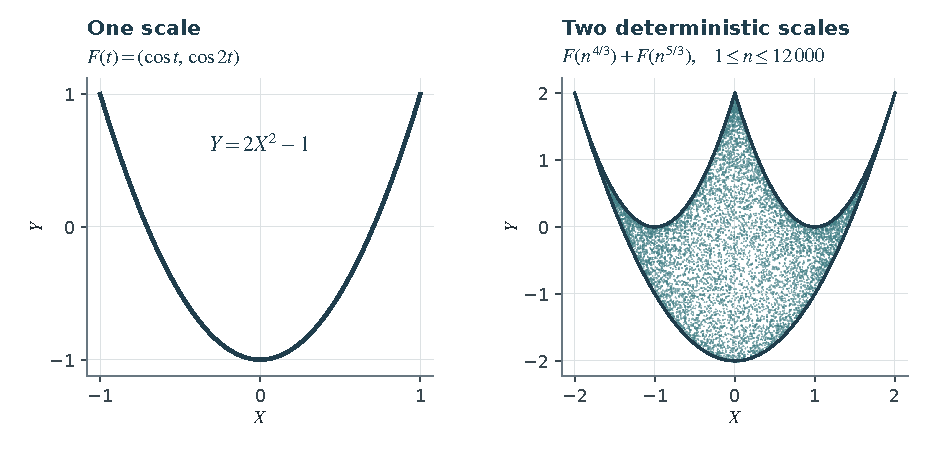
\includegraphics[width=.94\linewidth]{resonant-model.pdf}
\caption{A fully resonant model in two dimensions. One observation lies on \(y=2x^2-1\). The right panel uses \(12{,}000\) deterministic sums at exponents \(4/3\) and \(5/3\). Writing \(x=u+v,\ y=2(u^2+v^2)-2\) with \(u,v\in[-1,1]\) gives the two exact support boundaries shown. The plotted points illustrate the general sharpness example.}\label{fig:model}
\end{figure}

\begin{corollary}[Orderings in pooled centered races]\label{cor:order}
Let \(M=\int x\dd\mu_X(x)\). For each \(m\), choose \(\alpha_j=1+j/(m+1)\). The limiting frequency as \(n\to\infty\) of each strict coordinate ordering of \(S_n-mM\) exists. As \(m\to\infty\), it tends to the probability of the same ordering for a centered Gaussian with covariance \(\operatorname{Cov}(\mu_X)\). In particular every ordering occurs with positive limiting frequency for all sufficiently large fixed \(m\).
\end{corollary}
\begin{proof}
The boundary of an ordering cone is contained in a finite union of tie hyperplanes. Each has zero mass under any convolution by Theorem~\ref{th:local}. That theorem also gives strictly positive variance in every nonzero direction. Apply the multivariate central limit theorem to independent vectors with law \(\mu_X\); the convolution identity transfers the result to \eqref{eq:Sn}. A nondegenerate Gaussian assigns positive probability to each strict ordering and zero probability to its boundary. There are only finitely many orderings for fixed \(q\).
\end{proof}
